\documentclass{article}
\usepackage{enumerate}
\usepackage{color}
\usepackage{graphicx}
\usepackage{amsmath}
\usepackage{geometry}
\usepackage{setspace}
\usepackage{minted}
\geometry{left=2.54cm,right=2.54cm,top=2.54cm,bottom=2.54cm}
\begin{document}
\begin{spacing}{2.0}
\vspace*{0.25cm}
\hrulefill
\thispagestyle{empty}
\begin{center}
\begin{large}
\sc{UM--SJTU Joint Institute \vspace{0.3em} \\ Introduction to Operating Systems \\ (VE482)}
\end{large}

\hrulefill


\vspace*{5cm}
\begin{Large}
\sc{Homework 4}
\end{Large}
\vspace{2em}
\end{center}
\vfill

\begin{table}[h!]
\flushleft
\begin{tabular}{lll}
Name: Yu Xiao \hspace*{2em}&
ID: 518021910696 \hspace*{2em}\\

Date: Oct 29, 2021
\end{tabular}
\end{table}
\end{spacing}

\hfill

\newpage
\noindent\textbf{Ex.1} -- \textit{Simple questions}
\begin{enumerate}
	\item It is possible that when the clock interrupt occurs, the run-time system is at the point of blocking or unblocking a thread. This may lead to some unexpected behaviours.\\ \\
	One solution to this problem could be setting a flag when the run-time system is entered, so that the clock handler can see this and set its own flag. When the run-time system finishes its works, it can check the flag of the clock handler and see if there is a clock interrupt. If clock interrupt happened, it can call the clock handler now.\\
	\item It is possible to implement a thread package in user space in such a case, but the efficiency of such a thread package will not be good enough. Since there is no system call like \mintinline{c}{select}, we may set an alarm clock for each thread that want to execute a system call. If the call is blocked, the control would be returned back to the thread package.
\end{enumerate}

\noindent\textbf{Ex.2} -- \textit{Monitors}\\ \\
	The execution of \mintinline{c}{waituntil} will have to check the value of the bool variable repeatedly, which will waste more resources than using \mintinline{c}{wait} and \mintinline{c}{signal}.\\

\noindent\textbf{Ex.3} -- \textit{Race condition in Bash}
\begin{enumerate}
    \item The bash script is implemented as shown below.
    \begin{minted}{shell}
    #!/bin/bash
    FILE=./ex3.txt
    if [ ! -f $FILE ]; then
        echo 0 > $FILE
    fi
    for i in {1..20}
    do
        value=$(tail -n 1 $FILE)
        value=$((value + 1))
        echo $value >> $FILE
    done
    \end{minted}
    
    Run the script with following command
    \begin{minted}{shell}
    ./ex3_1.sh & ./ex3_1.sh
    \end{minted}
    \begin{figure}[htb]
        \centering
        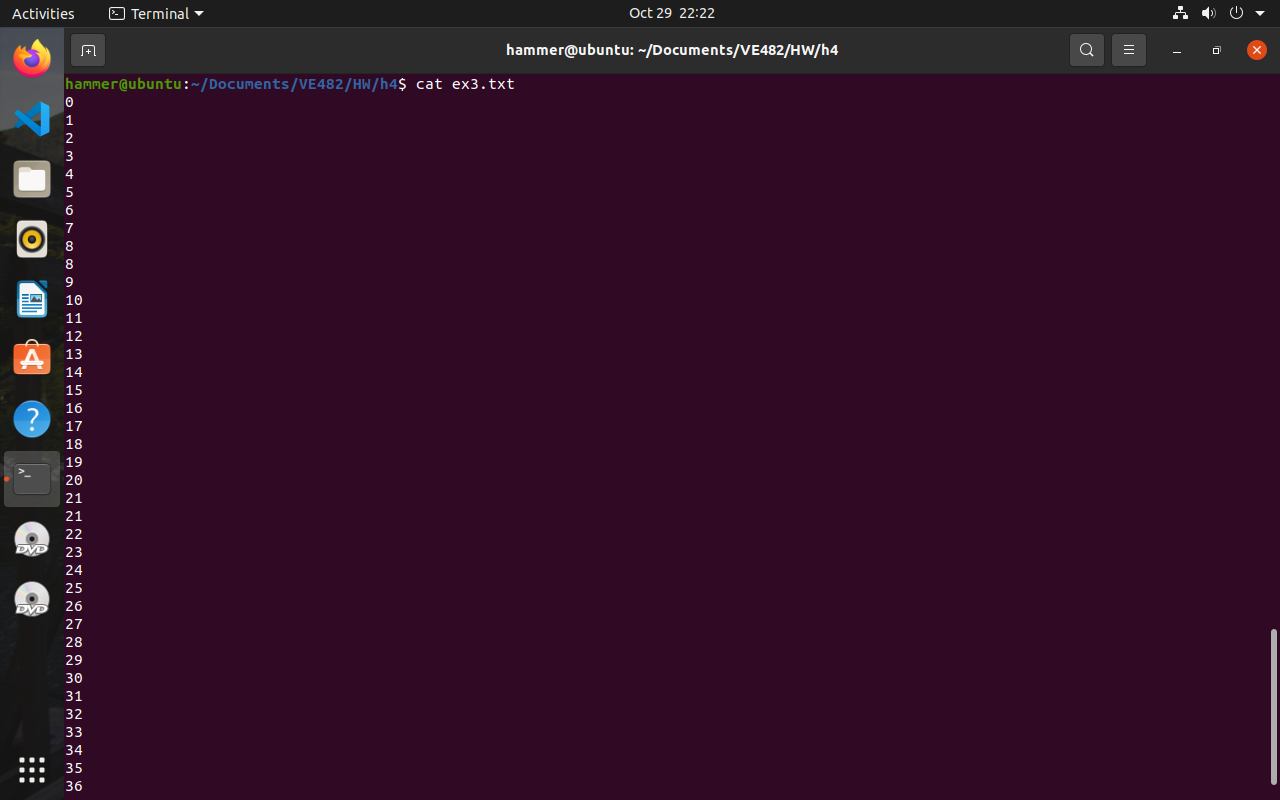
\includegraphics[width=0.8\linewidth]{ex3_1.png}
    \end{figure}
    In my own case, the race condition starts at the ninth line since there are two 8.
    \item Modified version is shown below.
    \begin{minted}{shell}
    #!/bin/bash
    FILE=./ex3.txt
    if [ ! -f $FILE ]; then
        echo 0 > $FILE
    fi
    for i in {1..20}
    do
        (
        flock -n -x 9
        value=$(tail -n 1 $FILE)
        value=$((value + 1))
        echo $value >> $FILE
        ) 9>>$FILE
    done
    \end{minted}
\end{enumerate}

\noindent\textbf{Ex.4} -- \textit{Programming with semaphores}\\ \\
For this exercise, please refer to \mintinline{shell}{./h4/cthread.c}
\begin{figure}[htb]
    \centering
    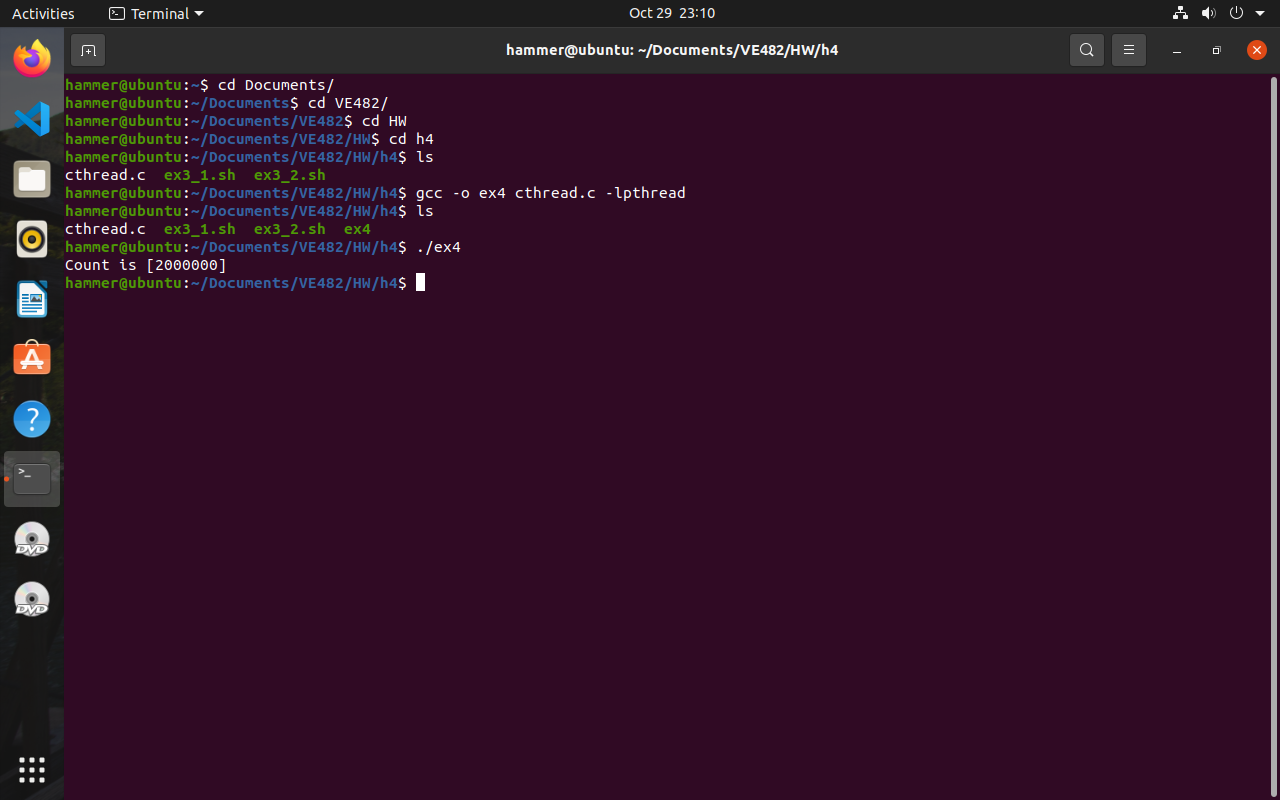
\includegraphics[width=0.8\linewidth]{ex4.png}
\end{figure}
\end{document}